\newpage
\chapter{Case Study Description}

To this day, Hydrogen trucks are starting to become a reality. 
What is proposed on the market or still under development offer values of  chassis occupation comparable with the ones of diesel-powered solutions.

Also the range of such solutions is in line with that is offered today in the fossil-fueled market: H2 tanks ranging from 30 to 100 kg can offer a range of more than 400 km \textsuperscript{\cite{pianoidrogeno}}.

A lot of effort in the development of Hydrogen powered trucks is being currently spent by joint-ventures between industies and logistic partners, like the partnership between \textbf{Scania} and \textbf{Asko}; given this fact, our case study will deal withthe analysis of the truck fleet needed by a sample logistic depot.

Our choice was the \textit{Amazon logistics depot in Milano}  (Via V. Toffetti 108). 
Being a pretty small depot, we imagined it to be served daily by \textbf{10} trucks.


The provision of Hydrogen to serve the daily needs of the depot has been performed analyzing the different solutions.
The focus is put on electrolysis with the energy produced by hydroelectric and photovoltaic plants.

In table \ref{tab:truckdata} we the have the data of Scania G-series truck. In image \ref{fig:electrolyser} we can see the chosen electrolyser \textsuperscript{\cite{2021HGas10MWSystem}}.
\begin{table}[ht!]
\centering
\begin{tabular}{|lc|}
\hline
\multicolumn{2}{|c|}{\cellcolor{bluepoli!40}{\textbf{Scania G series}}}                       \\ \hline
\multicolumn{1}{|l|}{WLTP Consumption {[}kg/km{]}}                     & $0,066$              \\ \hline
\multicolumn{1}{|l|}{Number of trucks}                                 & $5$                  \\ \hline
\multicolumn{1}{|l|}{Distance {[}km/day{]}}                            & $500$                \\ \hline
\multicolumn{1}{|l|}{Total $H_2$ required {[}kg/day{]}}                & $165$                \\ \hline
\multicolumn{1}{|l|}{LHV $H_2$ {[}kWh/kg{]}}                           & $33,31$              \\ \hline
\multicolumn{1}{|l|}{Electric energy required {[}MWh{]}}               & $8,456$              \\ \hline
\end{tabular}
\caption{Truck data}
\label{tab:truckdata}
\end{table}

\begin{figure}[h]
    \centering
    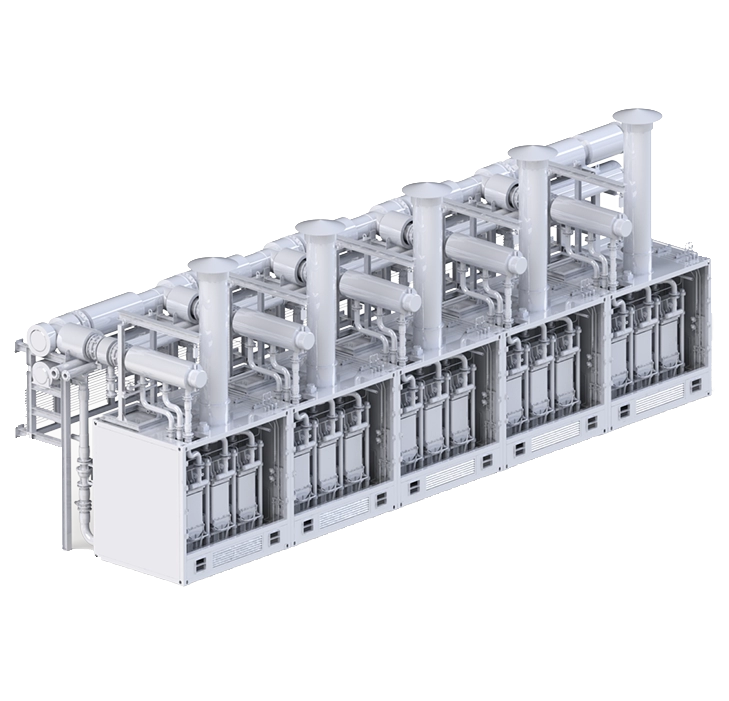
\includegraphics[width=0.6\textwidth]{Chapters/Pictures/Megastack-0X-5f524dc0.png}
    \caption{HgasXMW electrolyser}
    \label{fig:electrolyser}
\end{figure}
\begin{table}[h]
\centering
\begin{tabular}{|l|l|}
\hline
\rowcolor{bluepoli!40} \textbf{HGasXMW}                          & \textbf{Specs}                  \\ \hline
Ectrolyser technology                     & PEM                             \\ \hline
Number of stacks                          & 15                              \\ \hline
Electrolyser packaging                    & installation indoors            \\ \hline
Control                                   & PLC or DCS                      \\ \hline
Hydrogen purity                           & Up to $99,999\%$ (ISO standard) \\ \hline
Maximum hydrogen production appx (kg/24h) & $4050$                          \\ \hline
Input power at maximum appx (kW)          & $10070$                         \\ \hline
\end{tabular}
\caption{Tech Specs of HGasXMW}
\label{tab:specshydrolyser}
\end{table}

%\section{Logistic Depot}
\section{Hydroelectric power}
\subsection{Transport of Electricity, Electrolyser in the depot}

This first solution is based on these assumptions:

\begin{description}
    \item[\textbf{Electricity Production}]  Electricity is produced by the Hydroelectric PP in \textit{Crodo (VB)}. See table \ref{tab:crodotechspec} for techical data. Then the electricity is transfereed using the grid.
    \item[\textbf{Electrolysis}]  Electrolysis is performed on site in the depot, with a system owned by the logistics company.
\end{description}

\begin{table}[h]
\centering
\begin{tabular}{|lc|}
\hline
\rowcolor{bluepoli!40}\multicolumn{2}{|c|}{\textbf{Hydropower Plant - Crodo}}      \\ \hline
\multicolumn{1}{|l|}{Efficient power {[}kW{]}}                      & $52.800,00$  \\ \hline
\multicolumn{1}{|l|}{Distance from depot {[}km{]}}                  & $160,00$     \\ \hline
\multicolumn{1}{|l|}{V$_{Line}$ {[}V{]}}                            & $200.000,00$ \\ \hline
\multicolumn{1}{|l|}{I$_{Line}$ {[}A{]}}                            & $264,00$     \\ \hline
\multicolumn{1}{|l|}{Power loss {[}\%{]} (HV systems)}              & $0,02$       \\ \hline
\multicolumn{1}{|l|}{Effective power {[}kW{]}}                      & $51.744,00$  \\ \hline
\end{tabular}
\caption{\textit{Techinical data of \href{https://goo.gl/maps/dqKiAsYcyXrGMbUd6}{Crodo's Hydropower Plant}}}
\label{tab:crodotechspec}
\end{table}


%% Please add the following required packages to your document preamble:
% \usepackage[table,xcdraw]{xcolor}
% If you use beamer only pass "xcolor=table" option, i.e. \documentclass[xcolor=table]{beamer}
\begin{table}[hp]
\centering
\begin{tabular}{cc}
\hline
\rowcolor{bluepoli!40}\multicolumn{2}{|c|}{\cellcolor{bluepoli!40}\textbf{PEM electrolyzer near the depot}}                        \\ \hline
\multicolumn{1}{|c|}{\textbf{maximum H2 production {[}kg/h{]}}}          & \multicolumn{1}{c|}{36.00}       \\ \hline
\multicolumn{1}{|c|}{\textbf{hours to satisfy demand}}                   & \multicolumn{1}{c|}{5.04}        \\ \hline
\multicolumn{1}{|c|}{\textbf{Working hours {[}h{]}}}                     & \multicolumn{1}{c|}{8.00}        \\ \hline
\multicolumn{1}{|c|}{\textbf{max power {[}kW{]}}}                        & \multicolumn{1}{c|}{2,350.00}    \\ \hline
\multicolumn{1}{|c|}{\textbf{Prod to satisfy demand in 8h   {[}kg/h{]}}} & \multicolumn{1}{c|}{22.69}       \\ \hline
\multicolumn{1}{|c|}{\textbf{Actual Power {[}kW{]}}}                     & \multicolumn{1}{c|}{1,480.99}    \\ \hline
\multicolumn{1}{|c|}{\textbf{Energy {[}MWh{]}}}                          & \multicolumn{1}{c|}{11.85}       \\ \hline
\multicolumn{1}{|c|}{\textbf{mean UE distr. cost {[}€/kWh{]}}}           & \multicolumn{1}{c|}{0.03}        \\ \hline
\multicolumn{1}{|c|}{\textbf{Tot cost of electricity   {[}€/day{]}}}     & \multicolumn{1}{c|}{339.324}     \\ \hline
\multicolumn{1}{|c|}{}                                                   & \multicolumn{1}{c|}{}            \\ \hline
\multicolumn{1}{|c|}{\textbf{Mean investment cost {[}€/kW{]}}}           & \multicolumn{1}{c|}{1921.5}      \\ \hline
\multicolumn{1}{|c|}{\textbf{Investment cost {[}€{]}}}                   & \multicolumn{1}{c|}{2845721.484} \\ \hline
\multicolumn{1}{|c|}{\textbf{mean life of the plant {[}h{]}}}            & \multicolumn{1}{c|}{40000}       \\ \hline
\multicolumn{1}{|c|}{\textbf{mean life of plant {[}days{]}}}             & \multicolumn{1}{c|}{1667}        \\ \hline
\multicolumn{1}{|c|}{\textbf{Daily investment cost {[}€/day{]}}}         & \multicolumn{1}{c|}{1707}        \\ \hline
\multicolumn{1}{|c|}{\textbf{}}                                          & \multicolumn{1}{c|}{}            \\ \hline
\multicolumn{1}{|c|}{\textbf{TOT DAILY COST {[}€/day{]}}}                & \multicolumn{1}{c|}{2047}        \\ \hline
\end{tabular}
\caption{Provided solution with 10 trucks}
\label{tab:Crodo10Trucks}
\end{table}

\subsection{Far Electrolysis}
This second solution consist in the production of Hydrogen on the site of the Hydroelectri power plant of Trezzo sull'adda (see table \ref{tab:trezzoaddaspec}). Then the hydrogen is transfered by truck to the depot (cost $3,00$ €/kg\textsuperscript{\cite{pianoidrogeno}}) 
%\begin{table}[ht]
\centering
\begin{tabular}{|lc|}
\hline
\multicolumn{2}{|c|}{\cellcolor{bluepoli!40}Hydroelectric PP in Crodo}               \\ \hline
\multicolumn{1}{|l|}{Efficient power {[}kW{]}}                      & $52.800$       \\ \hline
\multicolumn{1}{|l|}{Distance from depot {[}km{]}}                  & $160$          \\ \hline
\multicolumn{1}{|l|}{$V_{line}$ {[}V{]}}                            & $200.000$      \\ \hline
\multicolumn{1}{|l|}{$I_{line}$ {[}A{]}}                            & $264$          \\ \hline
\multicolumn{1}{|l|}{Power loss percentage (HV systems)}            & $2\%$          \\ \hline
\multicolumn{1}{|l|}{Effective power {[}kW{]}}                      & $51.744$       \\ \hline
\multicolumn{2}{|c|}{\cellcolor{bluepoli!40}Electrolyzer near the depot}             \\ \hline
\multicolumn{1}{|l|}{$H_2$ request {[}kg/day{]}}                    & $181,50$       \\ \hline
\multicolumn{1}{|l|}{Maximum $H_2$ production {[}kg/h{]}}           & $36$           \\ \hline
\multicolumn{1}{|l|}{Maximum power {[}kW{]}}                        & $2.350$        \\ \hline
\multicolumn{1}{|l|}{Production to satisfy demand in 8h {[}kg/h{]}} & $22,6875$      \\ \hline
\multicolumn{1}{|l|}{Actual required power {[}kW{]}}                & $1480,99$      \\ \hline
\multicolumn{2}{|c|}{\cellcolor{bluepoli!40}Electric grid}                           \\ \hline
\multicolumn{1}{|l|}{Energy required {[}MWh{]}}                     & $11,85$        \\ \hline
\multicolumn{1}{|l|}{EU average energy cost {[}€/kWh{]}}            & $0,02864$      \\ \hline
\multicolumn{1}{|l|}{Total cost {[}€{]}}                            & $339,324$      \\ \hline
\end{tabular}
\caption{Hydroelectric power plant and electrolyzer near the depot}
\label{tab:secondsolution}
\end{table}
\begin{table}[hb!]
\centering
\begin{tabular}{|lc|}
\hline
\rowcolor{bluepoli!40}\multicolumn{2}{|c|}{\textbf{Hydroelectric Power plant - Trezzo Sull'Adda}} \\ \hline
\multicolumn{1}{|l|}{Efficient power {[}kW{]}}              & $10.500,00$                         \\ \hline
\multicolumn{1}{|l|}{Mean producible energy {[}kWh{]}}      & $65.000.000,00$                     \\ \hline
\multicolumn{1}{|l|}{Distance from depot {[}km{]}}          & $40,00$                             \\ \hline
\multicolumn{1}{|l|}{$V_{Line}$ {[}V{]}}                    & $200.000,00$                        \\ \hline
\multicolumn{1}{|l|}{$Current_{Line}$ {[}A{]}}              & $52,50$                             \\ \hline
\multicolumn{1}{|l|}{Power loss [\%] (HV systems)}          & $0,02$                              \\ \hline
\multicolumn{1}{|l|}{Effective power {[}kW{]}}              & $10.290,00$                         \\ \hline
\end{tabular}
\caption{Techinical data of \href{https://g.page/centrale-idroelettrica-taccani?share}{Trezzo sull'Adda Hydropower plant}}
\label{tab:trezzoaddaspec}
\end{table}



\section{PV}
Other two main solutions are the use of photovoltaic power plant to produce the energy required for the hydrogen. We continue to use the same eclectrolyser used befor (Figure \ref{fig:electrolyser}).

The distinction is on the place of the production (one in Puglia di other in Milan). In table \ref{tab:pvbessass} can be seen the assumption about the efficiency.

\begin{table}[h!]
\centering
\begin{tabular}{|lc|}
\hline
\rowcolor{bluepoli!40}\multicolumn{2}{|c|}{\textbf{Efficiency assumptions}}                 \\ \hline
\multicolumn{1}{|l|}{BESS Charging efficiency}   & \textbf{$0,95$}                          \\ \hline
\multicolumn{1}{|l|}{BESS Self discharge}        & \textbf{$0,90$}                          \\ \hline
\multicolumn{1}{|l|}{BESS discharge}             & \textbf{$0,97$}                          \\ \hline
\multicolumn{1}{|l|}{Plant efficiency}           & \textbf{$0,80$}                          \\ \hline
\multicolumn{1}{|l|}{RTE efficiency}             & \textbf{$0,83$}                          \\ \hline
\multicolumn{1}{|l|}{Energy required {[}MWh{]}}  & \textbf{$23,72$}                         \\ \hline
\end{tabular}
\caption{Phototovoltaic and BESS efficiency assumptions}
\label{tab:pvbessass}
\end{table}

\subsection{Photovoltaic Plant Puglia}
In this case we will use part of the projected Photovoltaic Plant in\href{https://goo.gl/maps/HDedbnQQh3Apqn599}{Troia(Puglia)} with the production on site of the hydrogen. Then it will be transfered to the depot by truck.

We will also analyse, in the next chapters, the economical sustainability of storage the energy and look if the storage of Hydrogen is more sustainable. In \ref{tab:hpuglia} we can see the irradiation coefficient \textsuperscript{\cite{PVINFOSYSTEM}}.

\begin{table}[h!]
\centering
\begin{tabular}{|l|l|c|}
\hline
\rowcolor{bluepoli!40} \textbf{Month} & \textbf{Days} & $\textbf{H }[kWh/m^2\cdot month]$ \\ \hline
1              & 31            & $105,68$       \\ \hline
2              & 28            & $108,01$       \\ \hline
3              & 31            & $125,45$       \\ \hline
4              & 30            & $176,99$       \\ \hline
5              & 31            & $193,44$       \\ \hline
6              & 30            & $187,80$       \\ \hline
7              & 31            & $215,53$       \\ \hline
8              & 31            & $204,94$       \\ \hline
9              & 30            & $165,46$       \\ \hline
10             & 31            & $135,13$       \\ \hline
11             & 30            & $121,34$       \\ \hline
12             & 31            & $112,82$       \\ \hline
\end{tabular}
\caption{\textit{Irradiation coefficient per month in Puglia\textsuperscript{\cite{PVINFOSYSTEM}}}}
\label{tab:hpuglia}
\end{table}
\begin{table}[p]
\centering
\begin{tabular}{|l|l|c|}
\hline
\rowcolor{bluepoli!40} \textbf{Month} & \textbf{Days} & \multicolumn{1}{l|}{\textbf{H}$[kWh/m^2\cdot month]$} \\ \hline
1              & 31            & $20,6$                          \\ \hline
2              & 28            & $33,9$                          \\ \hline
3              & 31            & $57,4$                          \\ \hline
4              & 30            & $90,9$                          \\ \hline
5              & 31            & $136,5$                         \\ \hline
6              & 30            & $145,2$                         \\ \hline
7              & 31            & $184,8$                         \\ \hline
8              & 31            & $184,4$                         \\ \hline
9              & 30            & $147,9$                         \\ \hline
10             & 31            & $85,4$                          \\ \hline
11             & 30            & $32,1$                          \\ \hline
12             & 31            & $22,5$                          \\ \hline
\end{tabular}
\caption{Irradiation coefficient per month in Milan}
\label{tab:hmilan}
\end{table}
\subsection{Photovoltaic Plant Milan}
In this other case the power plant is build up on the roof of the depot. In table \ref{tab:hmilan} we can see the irradiation coefficient for this case.
